\chapter[*先进智能体架构]{*先进 Transformer 架构与智能体架构}\label{chap:arch}

\begin{learningbox}
本章将介绍先进的 Transformer 架构与智能体架构。具体而言，学完本章后，你将能够：
\begin{itemize}[leftmargin=*, nosep]
    \item 理解{\em 图灵完备性（Turing-completeness）}的概念，并了解 Transformer 原则上具有图灵完备性。
    \item 理解当我们使用{\em 决策轨迹（decision traces）}而非自然语言来训练 Transformer 模型时，它们能够进行规划。
    \item 描述在{\em 循环式语言模型（looped language models）}中，如何跳过词元化层，将嵌入直接连接到其他嵌入。
    \item 描述智能体如何通过存储状态—动作—奖励三元组的历史记录，进行{\em 上下文强化学习（in-context reinforcement learning）}。
    \item 描述{\em 能够自我修改（self-modifying）}的智能体的优点与缺点。
    \item 理解如何将元学习应用于控制框架设计，创建能够改进基础控制框架的{\em 元控制框架（meta-harness）}。
\end{itemize}
\end{learningbox}

\section{Transformer 架构}
大语言模型的成功，为 Transformer 架构研究开辟了一些有趣的新方向。大语言模型擅长语言，却不擅长推理与规划等其他类型的问题。这促使研究者探索 Transformer 能够执行哪些计算，以及这些计算的边界；我们将在接下来的几节中讨论其中一些主题。具体而言，研究者提出了这样一个问题：Transformer 是否具有图灵完备性（第~\ref{sec:turing}~节）？它们在规划问题上的表现较弱，促使研究者直接使用决策轨迹来训练 Transformer，考察这样能否使其具备规划与回溯能力（第~\ref{sec:decisions}~节）。随后，我们将介绍循环式语言模型，其中多个模型在嵌入层面直接相连。


\subsection{Transformer 具有图灵完备性}\label{sec:turing}
大语言模型在推理阶段难以管理状态，这似乎表明，它们能够执行的计算类型是有限的。
在理论计算机科学中，图灵完备性这一概念用于说明：某种计算模型是否足够强大，能够执行某一类别中的任何计算，其中也包括正确管理状态值的能力。Alan Turing 在 1936 年的一篇著名论文中提出了这一概念，并证明某一类机器足够强大，能够做到这一点 \citep{turing1936computable}。
一个系统要被称为图灵完备的，就必须能够模拟任何其他计算设备，并处理任何能够用算法表达的问题，不过，这或许需要无限的时间与内存。
事实证明，实现图灵完备性并不太难；大多数通用编程语言都具有图灵完备性。\footnote{例如，Python 编程语言具有图灵完备性，而不含反向引用的简单正则表达式匹配则不具有图灵完备性。}

大语言模型以及一般的基于 Transformer 的模型都难以管理状态，这似乎意味着，Transformer 架构可能不具有图灵完备性。
有趣的是，早在 2021 年，\citet{perez2021attention} 就研究了这个问题，并证明 Transformer 架构能够模拟图灵机，因此具有图灵完备性。

这是一个令人鼓舞的结果，因为它表明，Transformer 无法正确管理状态，并没有根本性的原因。问题很可能在于找到合适的提示，或者合适的预训练与微调数据集。

遗憾的是，某件事在理论上可行，并不意味着实现它很容易，也不意味着能够高效地实现。
例如，对 Transformer 架构作出某些扩展，或许能够使高效的状态管理更容易实现。
下面，我们将讨论为使大语言模型能够高效解决决策与规划问题而开发的方法。


\subsection{在决策轨迹上预训练回溯能力}\label{sec:decisions}
Transformer 具有图灵完备性这一发现，推动了规划与决策方面的研究。
本节将讨论一些使用决策轨迹对 Transformer 架构进行预训练、并取得良好结果的研究。请注意，本节讨论的{\em 并非}在自然语言上训练的 Transformer，也就是大语言模型，而是在决策轨迹上训练的 Transformer。

\begin{figure}
    \centering
    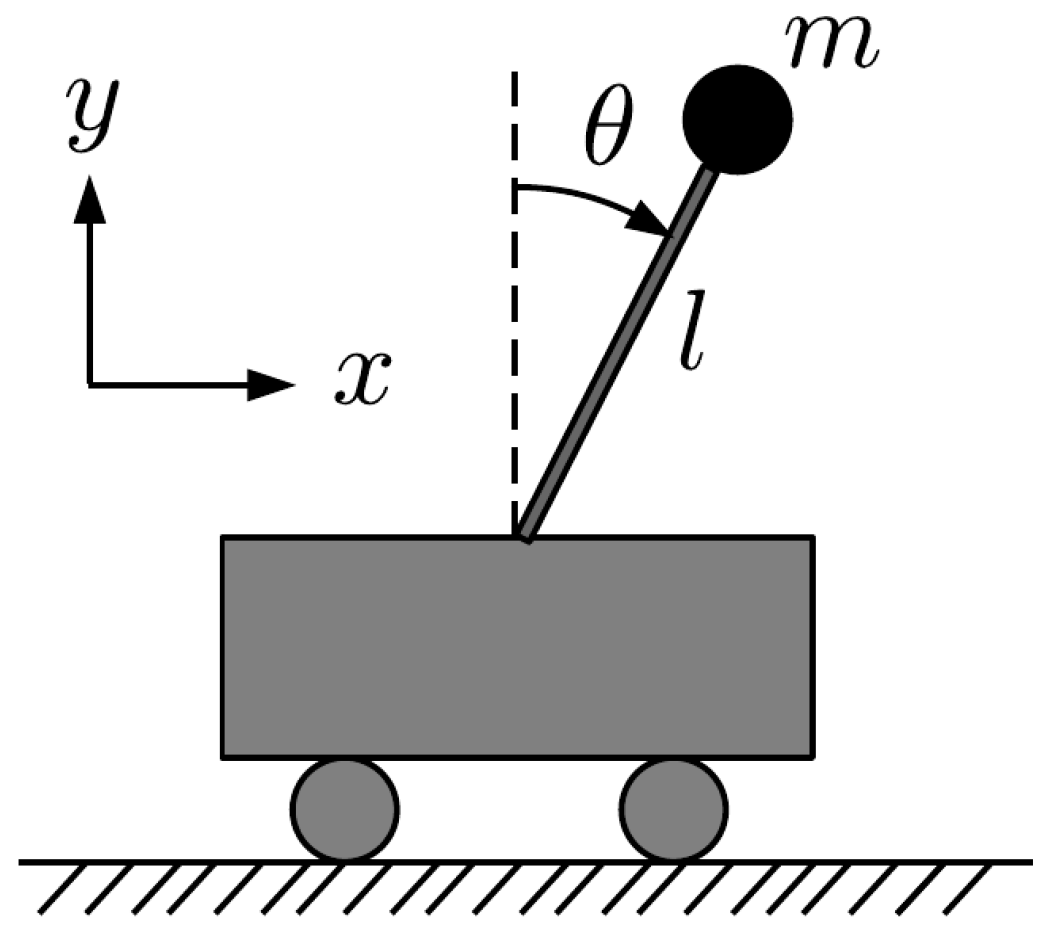
\includegraphics[width=0.5\linewidth]{figures/cartpole}
    \caption{倒立摆问题：仅通过向左或向右移动小车来保持杆的平衡}
    \label{fig:cartpole}
\end{figure}

首先，我们讨论直接在决策轨迹上预训练 Transformer。这些轨迹是状态—动作—奖励三元组序列，{\em 而非}语言词元。
多项研究考察了能否训练 Transformer 网络进行强化学习：从反馈中学习，执行学到的策略，并通过探索学会更好的动作。\citet{chen2021decision,lee2023supervised,wang2024transformers} 表明，基本的 Transformer 架构确实可以在典型规划问题的决策轨迹上进行预训练与微调。
当一个空白的、未接受语言训练的 Transformer 在决策轨迹上进行预训练时，它可以表现出上下文强化学习（ICRL）能力。目前，研究者已经在 Boyan 链和倒立摆等玩具问题上展示了这一点（见图~\ref{fig:cartpole}）。
此外，在国际象棋与 Hex 棋中，通过在极小极大（minimax）\citep{markeeva2024clrs,knuth1975analysis} 和蒙特卡洛树搜索（MCTS）\citep{browne2012survey} 的搜索轨迹上预训练决策 Transformer，研究者也取得了令人鼓舞的结果 \citep{schultz2024mastering,kempinski2025game}。Transformer 能够学会向前展望并搜索若干步。其他研究也报告了在黑白棋（Othello）中取得的可喜结果 \citep{li2023emergent,kempinski2025game,chen2025if}。

另一项研究 Transformer 架构如何通过训练来作出决策的工作，是{\em 自我回溯（self backtracking）}\citep{yang2026step}。这种方法同样使用决策轨迹训练模型。不过，它引入了一种新的词元 $<$backtrack$>$，提示模型在推理阶段进行显式回溯。模型在一个决策数据集上进行训练；当训练过程中遇到错误时，模型就会学习使用 $<$backtrack$>$ 词元，以寻找替代解。随后，这种回溯会在推理阶段执行。模型运行一个由扩展／回溯／选择组成的机制，从而考察当前状态下的其他解。

在 24 点游戏与迷宫导航等典型规划问题上，自我回溯方法与基于小型 DeepSeek-R1 和 Qwen3 的标准基线相比，取得了良好结果。通过引入一种新的词元和新的回溯功能，这种方法使增强后的 Transformer 模型能够执行搜索，模糊了训练与推理之间的界限。

这些结果令人鼓舞，不过，Transformer 在状态管理方面的弱点究竟解决到了什么程度，仍是一个开放问题。在更大规模的问题上于推理阶段执行 ICRL，仍是一个活跃的研究方向。


\subsection{循环式大语言模型与递归式多智能体系统}
提高 Transformer 的表达能力，使它们更接近一种通用编程架构。我们将讨论另外两项进展：循环式语言模型与递归系统。

在语言层面连接大语言模型智能体很容易：只需让它们使用各自都接受过训练的自然语言彼此交谈即可。不过，这需要进行多次词元化与反词元化，既耗费时间，也会在嵌入之间引入差异。我们能否绕过词元化器，直接连接嵌入，并在这一层面进行训练与推理？


\citet{giannou2023looped} 展示了循环式 Transformer 如何模拟基本计算器、基本线性代数库，以及采用反向传播的上下文学习算法。循环式 Transformer 的输入神经元直接连接到 Transformer 的输出神经元，后者可以来自同一模型，也可以来自另一模型。循环式 Transformer 是一种强大的架构，例如可参见 \citet{yang2023looped,saunshi2025reasoning,zhu2025scaling}。

嵌入到嵌入的直接连接又进一步发展为递归式多智能体系统（recursive multi-agent systems）\citep{yang2026recursive}。这种方法将异构智能体连接成一个协作循环，支持分布内的潜在思维生成，以及跨智能体的潜在状态传递。一种内外循环学习算法，即元学习（见第~\ref{chap:meta}~章），通过跨递归轮次共享的、基于梯度的信用分配，实现整个系统的联合优化。在数学、科学、医学、搜索和代码生成等基准测试上，使用四个智能体开展的实验展示了稳定的多智能体训练。与其他单智能体／多智能体基线及递归基线相比，准确率提高了几个百分点，推理速度提高到两倍，词元用量也按相近比例减少。

RecursiveMAS 的一项创新，是引入了两级递归连接（recursive-link）。训练多智能体系统很困难，因为梯度必须流经多个模型，这一过程可能变得不稳定。RecursiveMAS 冻结底层大语言模型的参数，只训练轻量的 RecursiveLink 模块，从而改善这一过程。训练分为两个阶段。


\section{智能体架构}
除了新的 Transformer 架构，智能体大语言模型研究也催生了先进的智能体架构。首先，我们将介绍上下文强化学习：当提示中给出状态—动作—奖励三元组的历史记录时，大语言模型能够改进策略。其次，我们将介绍能够自我修改的智能体，并讨论这一方法的优点与缺点。最后，我们将介绍元智能体。



\begin{figure}
  \begin{center}
    \input figures/rl
    \caption{供参考的标准强化学习循环：智能体学习由 $\theta$ 参数化的策略 $\pi_\theta$，其依据是环境针对智能体所采取的动作给出的反馈奖励 $r$；动作 $a$ 根据策略 $\pi_\theta$ 选择，如此循环 \citep{sutton2018reinforcement}}\label{fig:rl6}
  \end{center}
\end{figure}


\subsection{上下文强化学习}\label{sec:icrl}
回顾第~\ref{sec:rl}~节，强化学习的目标是计算出一种策略，为每个状态给出最优动作 \citep{sutton2018reinforcement}。
在向这一策略收敛的过程中，智能体在每个时间步都从环境反馈，也就是奖励中，学习这些动作。
这些奖励增强了智能体对策略在各状态下所选动作的信心（见图~\ref{fig:rl6}）。
前一节介绍的自我反思方法，为智能体控制框架借用了强化学习的许多思想。下面，我们将讨论利用上下文强化学习来优化提示的相关方法，其中由大语言模型来改进提示。





已有研究观察到，当外部提示优化器向大语言模型提供环境历史记录时，强化学习式的学习机制会直接在模型内部涌现：某些自我反思循环中的大语言模型能够改进策略。这一现象称为上下文强化学习（ICRL）\citep{song2025reward}，见图~\ref{fig:rl-icrl}。


\citet{krishnamurthy2024can} 提出，在语言上训练的通用大语言模型，能否在上下文中进行探索，又能否在上下文中从反馈中学习。此后，多项研究对这一问题给出了肯定回答 \citep{demircan2024sparse,song2025reward,moeini2025survey,monea2024llms,nie2024evolve,wang2024transformers}。

在 ICRL 中，外部控制框架迭代调用大语言模型，在上下文中向其输入动作、状态与奖励三元组序列（图~\ref{fig:rl-icrl}）。三元组的历史记录在每次迭代中不断增长。大语言模型相应地改进其隐式策略，每次迭代都给出越来越好的动作选择，因此，我们认为它在模型内部实现了强化学习的核心过程。

在 ICRL 中，智能体算法选择一个{\em 动作}，对一个步骤进行采样，并从环境获得一个回答，即一个{\em 状态}与{\em 奖励}对，见图~\ref{fig:rl-icrl}。马尔可夫决策过程（Markov decision process，MDP）是这样一种过程：计算下一状态所需的全部相关信息，都包含在前一状态及所采取的动作中。因此，提供给策略大语言模型的提示包含所有相关信息；它不断积累 $(s,a,r)$ 三元组的历史记录，大语言模型可以利用这些记录，改进为每个状态选择最佳动作的策略。
\begin{figure}[t]
  \begin{center}
    \input figures/rl-icrl
    \caption{ICRL：利用强化学习优化提示}\label{fig:rl-icrl}
  \end{center}
\end{figure}
在状态表示方面，回答的历史记录是一个自然的选择。不过，总体而言，如何将大语言模型的提示改进过程最好地建模为 MDP，仍是一个活跃的研究方向。

在 ICRL 中，智能体使用大语言模型实现策略函数。与自我反思控制框架一样，大语言模型也可以使用不同的提示来扮演环境的角色。

上下文强化学习发生在多轮提示控制框架中：环境大语言模型在当前轮生成回答之后，大语言模型会为自己刚刚生成的回答计算一个数值奖励。
下一轮，控制框架再次使用相同任务向智能体大语言模型提供提示，而此时的上下文由之前的回答与奖励组成。
随着上下文变长，智能体大语言模型的回答质量也会提高。
如同强化学习算法一样，大语言模型能够在推理阶段最大化数值奖励。\citet{song2025reward} 报告，在思维树的应用任务中，包括 24 点游戏、创意写作和 ScienceWorld，ICRL 方法得到了验证，其表现优于 Self Refine 和 Reflexion。


ICRL 过程在大语言模型内部是如何运作的？推理阶段，大语言模型在 Transformer 网络中执行前向传播，计算推理 token。研究发现，这次前向传播会隐式执行强化学习 \citep{wang2024transformers}。


换言之，权重内学习（in-weights learning）是指模型在训练阶段通过训练权重学会正确答案；上下文学习是指模型在推理阶段从上下文中提供的少样本示例中学会正确答案；而上下文强化学习则是指大语言模型利用一个不断增长的状态—动作—奖励三元组序列，通过（表面上的）强化学习学会正确答案，这一序列由模型自己通过推理产生。因此，当上下文中给出一系列提示或历史记录时，优化策略的强化学习算法就由大语言模型的前向传播，也就是推理步骤，隐式完成。


请注意，大语言模型既可以用于智能体，充当策略优化器，也可以用于环境，计算下一状态与奖励。为了确保智能体确实在学习，而没有意外利用环境的知识，最好为两者使用各自独立的大语言模型。这也是一个活跃的研究方向。








\subsection{能够自我修改的超智能体}
本书已经讨论了基于搜索算法与强化学习的自我反思提示改进器。这些外部算法的代码由人类研究者编写，在智能体学习时不会改变。提示改进的方式受到这些静态算法的限制。

大语言模型擅长修改与评判计算机代码 \citep{zhuge2024agent}。原则上，我们很容易要求它们为智能体提示控制框架，或者上下文强化学习控制框架生成代码。我们甚至可以要求大语言模型在某个具体问题实例上运行这些代码，再根据实验结果，要求它改进提示改进器的代码。
如果大语言模型善于利用实验结果编写提示改进代码，这一方法的效果就可能优于已发表文献中的标准方法。

自修改代码（self-modifying code），即在执行期间改变自身指令的计算机程序，在计算机科学中历史悠久 \citep{cai2007certified}，是条件分支语句的一种替代方案。许多计算机语言都支持它，从汇编语言到 Lisp \citep{abelson2022structure} 和 Python 都不例外。这是一种强大的方法，可以用于提高性能，例如即时编译（just-in-time compilation）\citep{ansel2011language}。不过，程序的可预测性会降低，这可能使查找程序错误变得困难，也会引发安全方面的担忧。因此，在程序可预测性十分重要的情况下，有时不建议采用这种方法。

能够自我修改的智能体的一项优点是开放性：它们能够不断改进自身，不受静态算法设定的固定边界限制 \citep{schmidhuber2007godel}。挑战在于如何安全地做到这一点 \citep{zhang2026darwingodelmachineopenended}。
在 Darwin-G\"odel-Machine-Hyperagents 中，作者将 (1) 解决目标任务的智能体与 (2) 修改自身及任务智能体的元智能体，整合为一个可编辑的程序。请注意，元层面的修改过程本身也可以编辑，因此支持自我修改。原则上，这不仅可以改进任务求解行为，也可以改进产生后续改进的机制 \citep{zhang2026hyperagents}。不过，这些实验并未实现完全开放，因为它们使用固定的任务分布，以及固定的父代选择与评估协议。

随着方法的开放性增强，一个看似矛盾的挑战随之出现：如何控制改进过程，确保它不会退化，而能持续进步 \citep{cemri2025multi,ecoffet2020open}。
一般而言，强大的元学习方法面临的问题，是如何保证学习过程稳定。强大的生成能力需要强大的评估能力，使适应过程能够契合环境。

\subsection{元智能体}
在许多自我反思方法中见到的元学习双层优化过程，可以作为智能体控制框架设计中的一项显式设计原则。近期已经出现了多种这样的架构。在这些设计中，内层学习循环由控制框架与大语言模型组成，外层学习循环则改进内层控制框架的配置。内层控制框架的配置通常负责提示管理、记忆管理、工具使用，以及安全与控制，可以用语言或代码表示。外循环分析内循环的执行轨迹，以改进内层控制框架的配置或代码。下面，我们将简要介绍其中一些方法。


能够自我改进的编程智能体（self improving coding agent）\citep{robeyns2025self} 基于能够自我修改的智能体这一思想。研究者展示，一个配备基本编程工具的智能体系统能够自主编辑自身。该方法提高了软件工程基准任务上的表现，将成绩从 17\% 大幅提升至 53\%。

\begin{figure}
    \centering
    % Original pixels retain every icon, number and arrow; only explanatory labels are covered.
\begingroup
\begin{tikzpicture}[x=0.0112716763cm,y=-0.0112716763cm,
  every node/.style={inner sep=0pt,outer sep=0pt,align=center,font=\sffamily\fontsize{9.5}{11}\selectfont}]
  \node[anchor=north west] at (0,0) {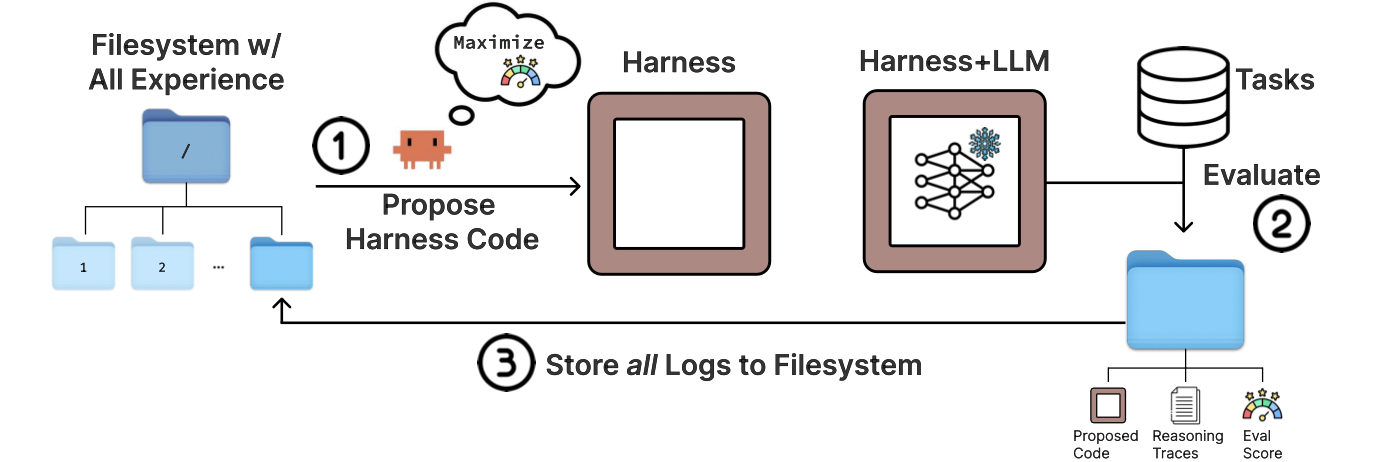
\includegraphics[width=15.6cm]{figures/metaharness.png}};
  \path[fill=white] (73,25) rectangle (313,99);
  \node[font=\sffamily\bfseries\fontsize{9.5}{11}\selectfont] at (194,62) {保存全部经验\\的文件系统};
  \path[fill=white] (450,29) rectangle (547,54);
  \node[font=\sffamily\bfseries\fontsize{7.5}{8.5}\selectfont] at (498,42) {最大化};
  \path[fill=white] (614,43) rectangle (775,80);
  \node[font=\sffamily\bfseries\fontsize{10}{11}\selectfont] at (683,62) {控制框架};
  \path[fill=white] (849,40) rectangle (1056,83);
  \node[font=\sffamily\bfseries\fontsize{9.5}{11}\selectfont] at (953,62) {控制框架＋LLM};
  \path[fill=white] (1232,60) rectangle (1332,96);
  \node[font=\sffamily\bfseries\fontsize{10}{11}\selectfont] at (1281,79) {任务};
  \path[fill=white] (336,192) rectangle (582,258);
  \node[font=\sffamily\bfseries\fontsize{9.5}{11}\selectfont] at (462,224) {提出\\控制框架代码};
  \path[fill=white] (1197,157) rectangle (1353,192);
  \node[font=\sffamily\bfseries\fontsize{10}{11}\selectfont] at (1272,176) {评估};
  \path[fill=white] (543,347) rectangle (1030,387);
  \node[font=\sffamily\bfseries\fontsize{9.5}{11}\selectfont] at (785,368) {将全部日志存入文件系统};
  \path[fill=white] (1065,428) rectangle (1147,462);
  \path[fill=white] (1149,428) rectangle (1228,462);
  \path[fill=white] (1237,428) rectangle (1307,462);
  \node[font=\sffamily\fontsize{7.5}{8}\selectfont] at (1107,463) {提出的\\代码};
  \node[font=\sffamily\fontsize{7.5}{8}\selectfont] at (1188,463) {推理\\轨迹};
  \node[font=\sffamily\fontsize{7.5}{8}\selectfont] at (1271,463) {评估\\得分};
\end{tikzpicture}
\endgroup

    \caption{Meta Harness 方法示意图 \citep{lee2026meta}}
    \label{fig:metaharness}
\end{figure}

Meta Harness \citep{lee2026meta} 使用外部记忆与文本优化，也取得了良好结果。图~\ref{fig:metaharness} 展示了它的工作方式。(1) 文件系统保存此前所有候选方案的源代码、执行轨迹与得分；智能体读取这些内容，为新的控制框架生成代码。(2) 在评估任务上评估提出的控制框架。(3) 将所有提出的代码、推理轨迹与评估得分存入文件系统中的一个新目录，然后重复这一循环。

Self Harness \citep{zhang2026self} 和 Agentic Harness Engineering \citep{lin2026agentic} 进一步探索了控制框架设计，在软件工程任务上取得了显著改进。能够递归自我演化的智能体（recursive self-evolving agents）\citep{nguyen2026recursive} 则侧重于能够自我改进的智能体中的选择环节。

\citet{luo2026autodesign} 描述了另一个应用场景。他们使用元控制框架，设计出将科学论文转化为会议海报的控制框架。因此，这项工作在两个层面作出了贡献：一种构建元控制框架的方法，以及一个用于设计海报的具体控制框架；作者自然也将它用于自己的论文。

\begin{figure}
    \centering
    % Reflow the original figure into three rows. Pixel-exact crops preserve icons, code and data.
\begingroup
\definecolor{ch20teal}{RGB}{28,118,123}
\definecolor{ch20violet}{RGB}{153,99,240}
\definecolor{ch20flowbg}{RGB}{250,247,255}
\begin{tikzpicture}[x=0.0135514019cm,y=-0.0135514019cm,
  every node/.style={inner sep=0pt,outer sep=0pt,align=center,font=\sffamily\fontsize{10}{11.5}\selectfont}]
  \node[anchor=north west] at (0,0) {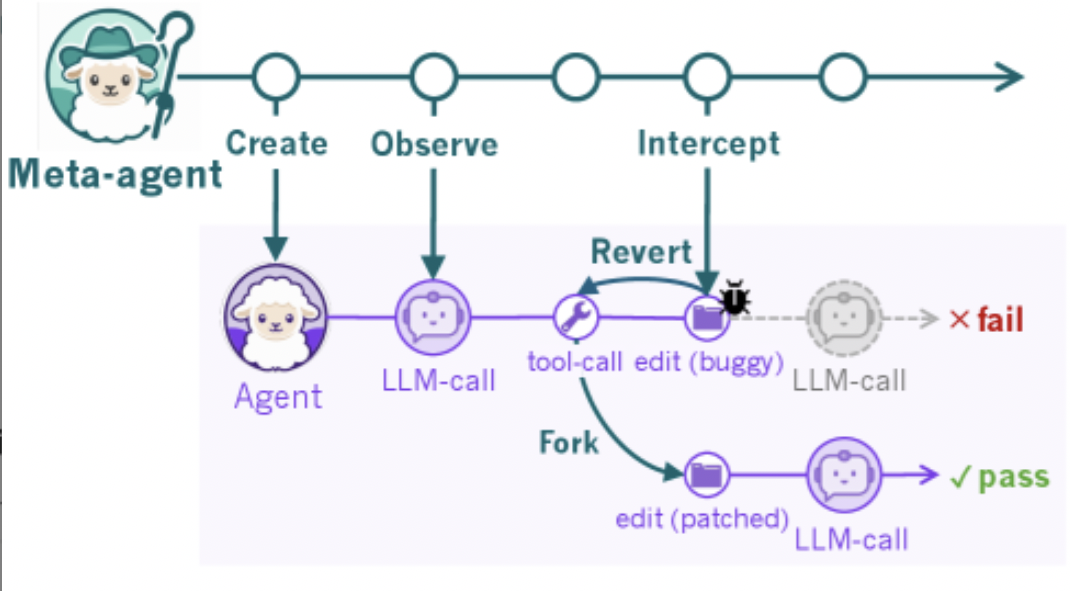
\includegraphics[width=14.5cm]{figures_zh/ch20/shepherd_flow.png}};
  \path[fill=white] (0,0) rectangle (3,591);
  \path[fill=white] (3,150) rectangle (226,205);
  \node[text=ch20teal,font=\sffamily\bfseries\fontsize{11}{12}\selectfont] at (111,175) {元智能体};
  \path[fill=white] (220,124) rectangle (334,160);
  \path[fill=white] (365,124) rectangle (507,160);
  \path[fill=white] (631,121) rectangle (789,166);
  \node[text=ch20teal,font=\sffamily\bfseries\fontsize{10}{11.5}\selectfont] at (278,143) {创建};
  \node[text=ch20teal,font=\sffamily\bfseries\fontsize{10}{11.5}\selectfont] at (435,143) {观测};
  \node[text=ch20teal,font=\sffamily\bfseries\fontsize{10}{11.5}\selectfont] at (709,143) {拦截};
  \path[fill=ch20flowbg] (229,376) rectangle (332,415);
  \node[text=ch20violet] at (280,396) {智能体};
  \path[fill=ch20flowbg] (587,233) rectangle (698,269);
  \node[text=ch20teal,font=\sffamily\bfseries\fontsize{10}{11.5}\selectfont] at (642,251) {回滚};
  \path[fill=ch20flowbg] (377,364) rectangle (505,398);
  \node[text=ch20violet,font=\sffamily\fontsize{9.5}{11}\selectfont] at (440,381) {LLM 调用};
  \path[fill=ch20flowbg] (521,347) rectangle (631,377);
  \node[text=ch20violet,font=\sffamily\fontsize{9}{10}\selectfont] at (576,362) {工具调用};
  \path[fill=ch20flowbg] (633,347) rectangle (791,377);
  \node[text=ch20violet,font=\sffamily\fontsize{8.5}{10}\selectfont] at (712,362) {编辑（有缺陷）};
  \path[fill=ch20flowbg] (792,364) rectangle (922,398);
  \node[text=gray,font=\sffamily\fontsize{9.5}{11}\selectfont] at (856,381) {LLM 调用};
  \path[fill=ch20flowbg] (975,300) rectangle (1057,339);
  \node[text=red!75!black,font=\sffamily\bfseries\fontsize{10}{11.5}\selectfont] at (1015,320) {失败};
  \path[fill=ch20flowbg] (530,427) rectangle (605,462);
  \node[text=ch20teal,font=\sffamily\bfseries\fontsize{9.5}{11}\selectfont] at (565,444) {派生分支};
  \path[fill=ch20flowbg] (612,504) rectangle (791,536);
  \node[text=ch20violet,font=\sffamily\fontsize{9}{10}\selectfont] at (704,519) {编辑（已修补）};
  \path[fill=ch20flowbg] (792,527) rectangle (923,558);
  \node[text=ch20violet,font=\sffamily\fontsize{9.5}{11}\selectfont] at (856,542) {LLM 调用};
  \path[fill=ch20flowbg] (976,459) rectangle (1062,500);
  \node[text=green!50!black,font=\sffamily\bfseries\fontsize{10}{11.5}\selectfont] at (1018,479) {通过};
\end{tikzpicture}
\par\vspace{2mm}
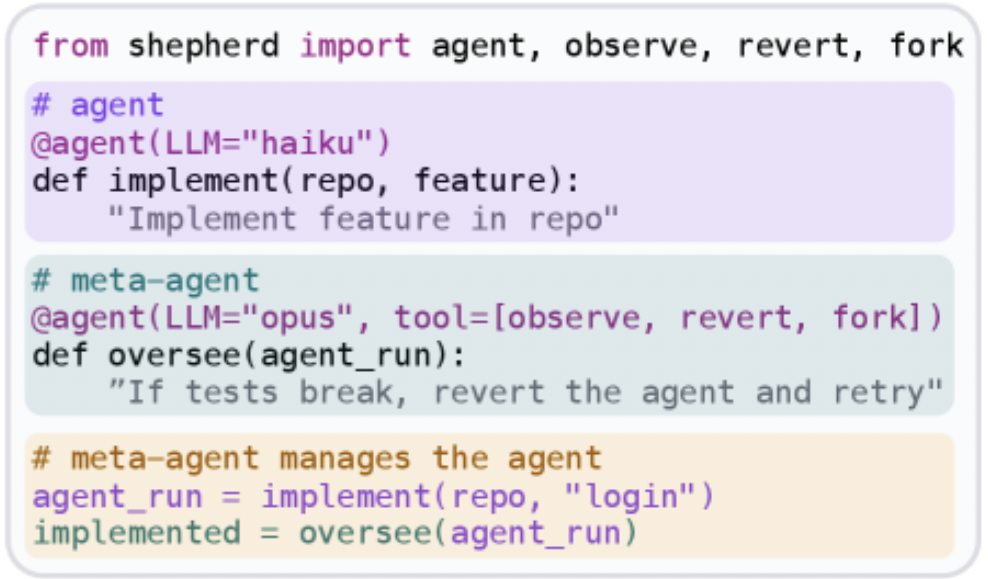
\includegraphics[width=12.5cm]{figures_zh/ch20/shepherd_code.png}
\par\vspace{2mm}
\begin{tikzpicture}[x=0.0075480769cm,y=-0.0075480769cm,
  every node/.style={inner sep=0pt,outer sep=0pt,align=center,font=\sffamily\fontsize{7.5}{8.5}\selectfont}]
  \node[anchor=north west] at (0,0) {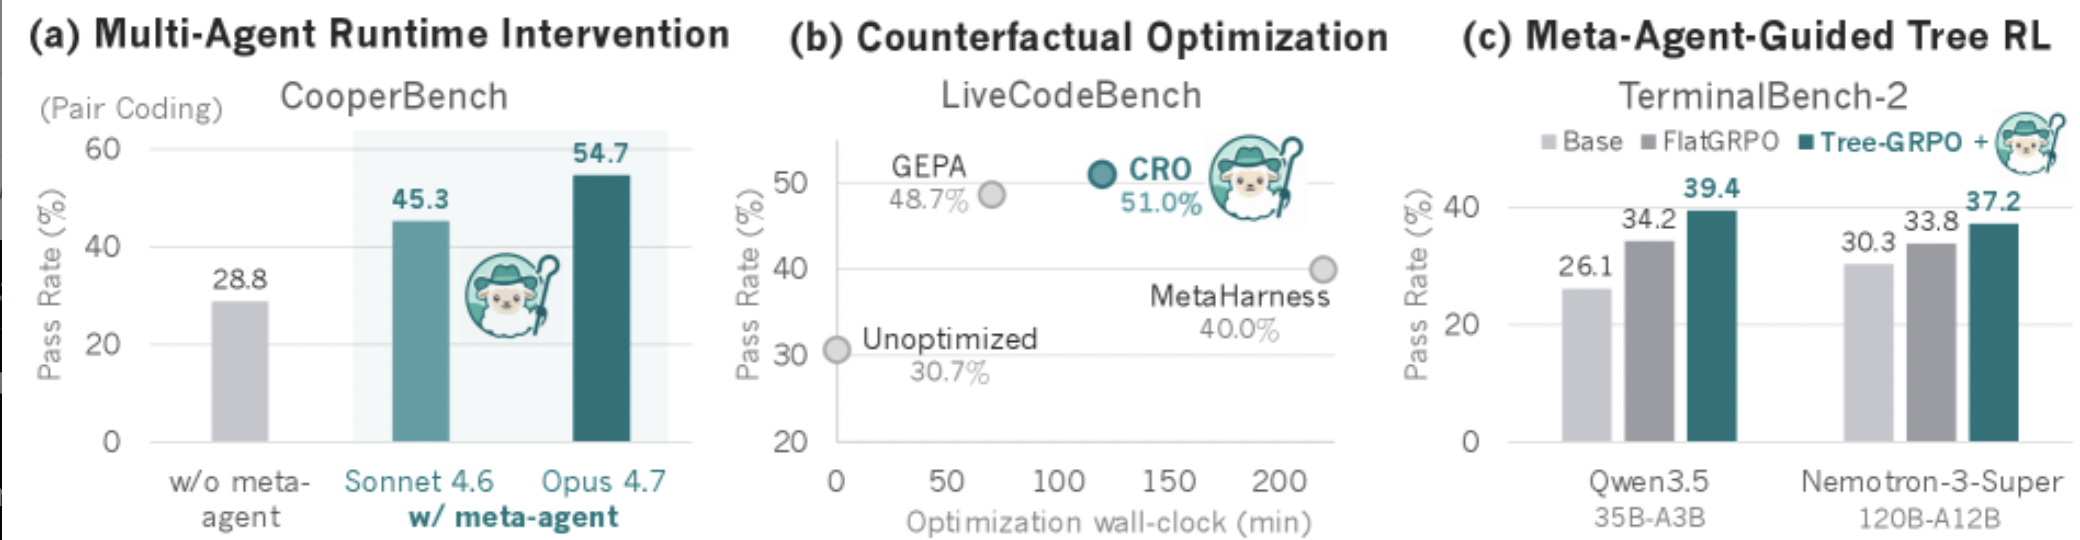
\includegraphics[width=15.7cm]{figures_zh/ch20/shepherd_charts.png}};
  \path[fill=white] (0,0) rectangle (3,540);
  \path[fill=white] (20,11) rectangle (742,60);
  \path[fill=white] (782,11) rectangle (1394,60);
  \path[fill=white] (1454,11) rectangle (2070,60);
  \node[font=\sffamily\bfseries\fontsize{8}{9}\selectfont] at (381,34) {(a) 多智能体运行时干预};
  \node[font=\sffamily\bfseries\fontsize{8}{9}\selectfont] at (1088,34) {(b) 反事实优化};
  \node[font=\sffamily\bfseries\fontsize{8}{9}\selectfont] at (1762,34) {(c) 元智能体引导的树式强化学习};
  \path[fill=white] (37,91) rectangle (230,126);
  \node at (133,109) {（结对编程）};
  \path[fill=white] (30,185) rectangle (69,384);
  \path[fill=white] (733,185) rectangle (771,384);
  \path[fill=white] (1398,185) rectangle (1437,384);
  \node[rotate=90] at (48,284) {通过率（\%）};
  \node[rotate=90] at (752,284) {通过率（\%）};
  \node[rotate=90] at (1410,284) {通过率（\%）};
  \path[fill=white] (164,465) rectangle (314,539);
  \node at (239,499) {无元智能体};
  \path[fill=white] (380,502) rectangle (666,539);
  \node[text=ch20teal,font=\sffamily\bfseries\fontsize{7.5}{8.5}\selectfont] at (523,520) {使用元智能体};
  \path[fill=white] (860,318) rectangle (1067,357);
  \draw[draw={rgb,255:red,235;green,235;blue,235},line width=0.3pt] (860,350) -- (1067,350);
  \node at (961,331) {未优化};
  \path[fill=white] (887,506) rectangle (1329,540);
  \node at (1108,523) {优化实际耗时（分钟）};
  \path[fill=white] (1560,126) rectangle (1626,158);
  \node at (1593,142) {基础};
\end{tikzpicture}
\endgroup

    \caption{Shepherd 元智能体环境示意图 \citep{yu2026shepherd}}
    \label{fig:shepherd}
\end{figure}

Shepherd 系统 \citep{yu2026shepherd} 提供了一个基于函数的元智能体编程环境。\footnote{\url{https://shepherd-agents.ai}} Shepherd 将大语言模型智能体定义为 Python 函数，使智能体的执行轨迹能够被监控、回滚、派生分支、修改和恢复执行。如图~\ref{fig:shepherd} 所示，早期实验在三个不同的基准测试上展示了显著的性能提升。

\citet{ren2026self} 提供了一篇综合综述，介绍了更多能够自我改进的智能体设计方法。其分类体系明确承认了这种双层架构。

\section{结语}
本章讨论了 Transformer 层面与智能体层面的一些先进架构。这两个领域的研究都十分活跃。

\bibliographystyle{plainnat}
\bibliography{agenticbook,refs,case,synthetic}

